\chapter{Evaluation}


\section{Connectivity Manager Integration with NUBOMEDIA project}

% % CM deliverable % %

The Connectivity Manager (CM) is part of the NUBOMEDIA platform and is placed between the virtual network resource management of the cloud infrastructure and the
multimedia application. The main focus of the CM is related to management and control of network functions of the virtual network infrastructure provided by OpenStack.

Nubomedia is an elastic Platform-as-a-Service (PaaS) cloud for interactive multimedia services \cite{nubomedia}. Its architecture is based on media pipelines: chains of elements providing media capabilities such as encryption, transcoding, augmented reality or video content analysis. These chains allow building arbitrarily complex media processing for applications. As a unique feature, from the point of view of the pipelines, the NUBOMEDIA cloud infrastructure behaves as a single virtual super-computer encompassing all the available resources of the underlying physical network. A big part of currently developed applications within the platform make use of WebRTC, which can use TCP or UDP traffic. This is why both protocols need to be evaluated.

\section{Network Performance Analysis}

The following section contains information about the used configuration followed by the different scenarios that were used to evaluate the effectiveness of the Connectivity Manager. All scenarios used the same topology and were deployed on a tenant without any other running servers or Heat stacks. The bandwidth tests were performed using the iperf tool.

\subsection{Test-bed Configuration}

The testbed consists of two nodes with the following hardware characteristics:

\begin{table}[H]
\centering

\begin{tabularx}{\textwidth}{ |X|X|X| }
\hline Name & \textbf{Control node} & \textbf{Compute node} \\ 
\hline Hostname & datacenter-4 & dc4-comp \\ 
\hline RAM & 12 GB & 8 GB \\ 
\hline CPU & 8-core Intel Core i7-4765T CPU @ 2.00GHz & 4-core Intel Core i3-2120T CPU @ 2.60GHz \\ 
\hline OS & Ubuntu 14.04.1 LTS & Ubuntu 14.04.1 LTS \\ 
\hline Kernel version & GNU/Linux 3.13.0-32-generic & GNU/Linux 3.13.0-32-generic \\
\hline Ethernet card & Intel Corporation Gigabit Ethernet Connection I217-LM & Intel Corporation 82579LM Gigabit Network Connection \\ 
\hline 
\end{tabularx}

\caption{Hardware resources of testbed used for evaluation}
\end{table}


The two nodes are connected to a Gigabit-Ethernet switch. The installation of OpenStack was performed using the devstack script as outlined in the Devstack section in the Implementation chapter.

\subsection{Installation of Connectivity Manager Agent}

A setup script exists in order to make it easier to get the CM Agent running. It builds and installs all the necessary Python packages in a virtual environment.This has the benefit that all packages are isolated from already existing Python installations and ensures that all packages are in the required version and don't interfere with the ones that are needed by OpenStack or other applications. 

First of all the git repository needs to be cloned from the remote git server. For the installation the cm-agent.sh script needs to be executed with the 'install' option.

\textit{\$ ./cm-agent.sh}
\begin{lstlisting}
Usage: cm-agent.sh option
options:
  install   - install the server
  update    - updates the server
  start     - start the server
  uninstall - uninstall the server
  clean     - remove build files
\end{lstlisting}
The installation process includes setting up the virtual environment, installing all required Python packages and copying the configuration file to the /etc/nubomedia folder.

The configuration file needs to be customized, so it contains the IP address of the control node and the correct OpenStack tenant credentials:

\textit{\$ cat /etc/nubomedia/cm-agent.properties:}
\begin{lstlisting}
os_username=admin
os_password=pass
os_auth_url=http://192.168.41.45:5000/v2.0
os_tenant=demo
\end{lstlisting}

Lastly it can be run in a screen session using the following command: \\
\textit{\$ venv/bin/python cm-agent/wsgi/application.py}

\subsection{Topology Definition}

The topology that is used for the evaluation contains the following services instances:

\textit{data/json\_file/topologies/topology\_local.json:}
\begin{lstlisting}[language=json,firstnumber=1]
{
    "name":"local_nm_template_minified",
    "service_instances": [
        {
            "name":"Controller",
            "service_type":"Controller"
        },
        {
            "name":"Broker",
            "service_type":"Broker"
        },
        {
            "name":"MediaServer",
            "service_type":"MediaServer"
        }
    ]
}
\end{lstlisting}

It can be deployed using a test application which performs a HTTP POST to the EMM API at the \textit{/topologies} path.

The service types are further defined in another JSON file, which includes their configuration, networks and other parameters that are needed for provisioning. As one example the Media Server service is given below:

\textit{data/json\_file/services/MediaService.json:}
\begin{lstlisting}[language=json,firstnumber=1]
{
    "service_type": "MediaServer",
    "version":"1",
    "image": "trusty-iperf",
    "flavor": "m1.mini",
    "key":"nubomedia",
    "configuration": {
    },
    "size": {
        "min": 1,
        "def": 3,
        "max": 5
    },
    "networks": [
        {
            "name":"Network-1",
            "private_net":"8048fd67-70a6-447d-a779-8a86f9eeb35d",
            "private_subnet": "0df3f54c-d1af-4b82-8376-18baa11d0e98",
            "public_net": "62024eab-23c2-4a81-a996-87af4d252282",
            "security_groups": [
                "SecurityGroup-MediaServer"
            ]
        }
    ],
    "requirements": [
        {
            "name":"$BROKER_IP",
            "parameter":"private_ip",
            "source":"Broker",
            "obj_name": "Network-1"
        }
    ]
}
\end{lstlisting}

\subsection{Scenario 1: Without Instance Placement Engine \& QoS enabled}

In this first scenario the deployment without any influence of the Connectivity Manager is shown. Here Nova randomly decides about the placement of the servers. In this case 4 servers were placed on the control node and one server on the compute node.

\begin{figure}[H]
\centering

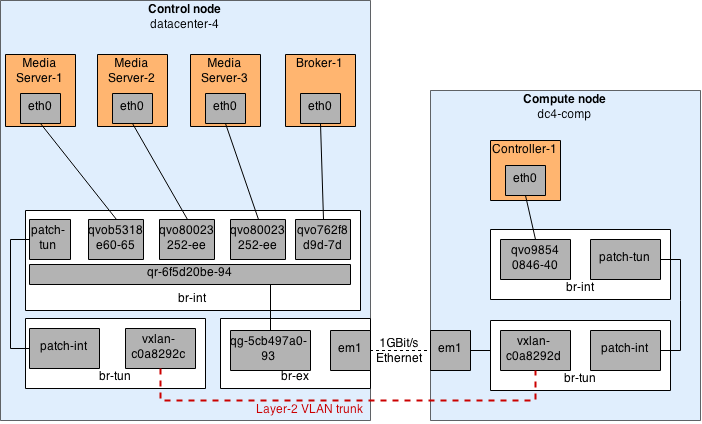
\includegraphics[width=0.7\textwidth]{images/evaluation/testbed_scenario1}

\caption{Scenario 1: Placement of servers without Connectivity Manager}
\end{figure}

\textbf{TCP traffic}

For testing the bandwidth the MediaServer-2 was used as a TCP server using iperf. All other servers connected to it in client mode sending and retrieving TCP packets in a timeframe of 10 seconds. The following graph shows the bandwidth usage of the servers.

\begin{figure}[H]
\centering

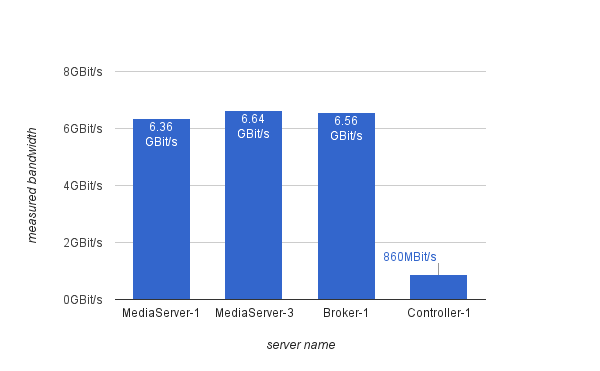
\includegraphics[width=0.5\textwidth]{images/evaluation/testbed_scenario1_bw}

\caption{Scenario 1: TCP Bandwidth comparison}
\end{figure}

As visible the network performance of the server on the separate node performs much worse, which is also due to the fact that there is only a Gigabit-Ethernet connection between the nodes.

\textbf{UDP traffic}

In order to test the bandwidth with UDP traffic, two servers where started as a UDP server and each of them received one client connection. The selected bandwidth limit that the packets were streamed at is 800 MBit/s.

\begin{table}[H]
\centering

\begin{tabularx}{\textwidth}{ |X|X|X|X|X| }
\hline Server name & Measured bandwidth & Ratio lost/total datagrams & Datagrams out of order & Jitter \\ 
\hline MediaServer-1 & 780 MBit/s & 3.4\% & 18 & 0.011 ms\\ 
\hline Controller-1 & 779 MBit/s & 2\% & 49689 & 0.078 ms \\ 
\hline 
\end{tabularx}

\caption{Scenario 1: Network characteristics with generated UDP traffic}
\end{table}

The comparison of the network statistics shows that while the measured bandwidth is the same across all connections, even for the server that is located on the separate compute node, however the datagrams that are received by the server out of order is tremendously larger. Multiple tests showed also that the jitter is always of a bigger value, even though with only a minimal difference.


\subsection{Scenario 2: With Instance Placement Engine enabled, but without QoS}

In this next scenario, the Instance Placement Engine was enabled and therefore the availability zone in the topology was successfully set to a single host.

\begin{figure}[H]
\centering

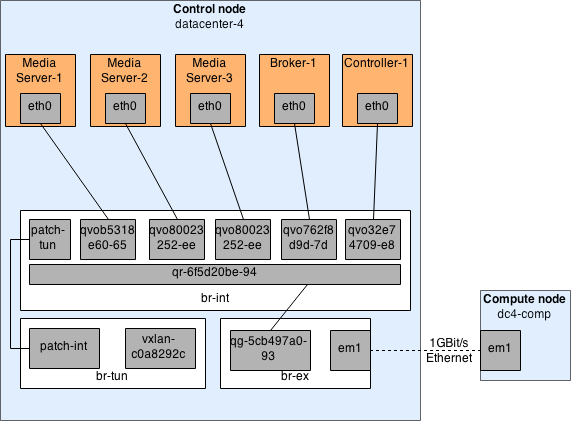
\includegraphics[width=0.7\textwidth]{images/evaluation/testbed_scenario2}

\caption{Scenario 2: Placement of servers with Connectivity Manager}
\end{figure}

\textbf{TCP traffic}

The following graph shows that the available bandwidth using TCP packets is now evenly distributed for all servers. However the traffic of the MediaServers should be prioritized, which is why QoS is needed to further improve the connectivity according to the requirements.

\begin{figure}[H]
\centering

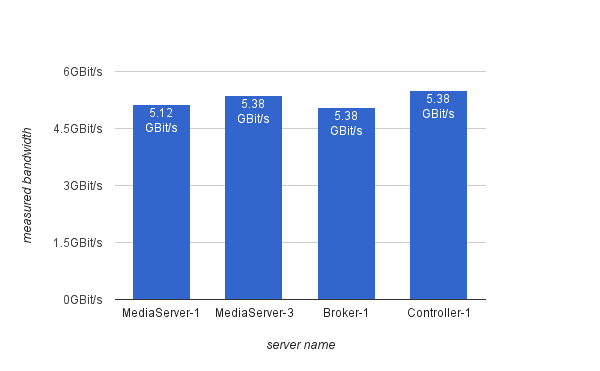
\includegraphics[width=0.5\textwidth]{images/evaluation/testbed_scenario2_bw}

\caption{Scenario 2: Bandwidth comparison}
\end{figure}

\textbf{UDP traffic}

The traffic generation was configured in the same way as in Scenario 1, except that now all servers are deployed on the same compute node.

\begin{table}[H]
\centering

\begin{tabularx}{\textwidth}{ |X|X|X|X|X| }
\hline Server name & Measured bandwidth & Ratio lost/total datagrams & Datagrams out of order & Jitter \\ 
\hline MediaServer-1 & 791 MBit/s & 2.3\% & 9 & 0.018 ms\\ 
\hline Controller-1 & 789 MBit/s & 2.7\% & 13 & 0.013 ms \\ 
\hline 
\end{tabularx}

\caption{Scenario 2: Network characteristics with generated UDP traffic}
\end{table}

With the servers all running on the same compute node, the datagrams that were received out of order could be minimized.

\subsection{Scenario 3: Instance Placement Engine and QoS Manager enabled}

The servers are again placed on a single host and the Quality of Service configuration that was previously set in the configuration is applied. All media servers have a guaranteed bandwidth rate of 100 MBit/s and a maximum rate of 10 GBit/s, while all servers of other instance types have a rate between 100 MBit/s and 1 GBit/s.

\begin{figure}[H]
\centering

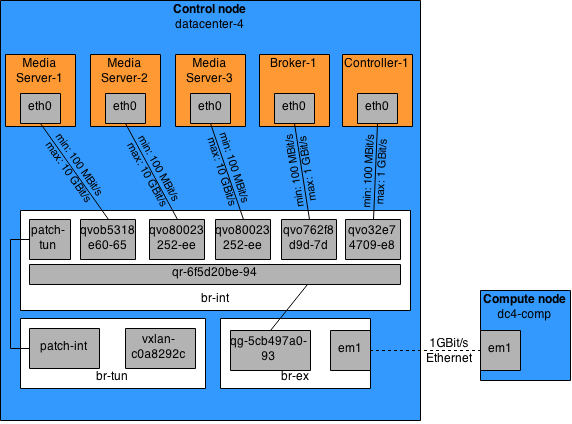
\includegraphics[width=0.7\textwidth]{images/evaluation/testbed_scenario3}

\caption{Scenario 3: Placement of servers using the Connectivity Manager with QoS enabled}
\end{figure}

The topology with it's configured QoS Queues is also visible by performing a HTTP GET to the Connectivity Manager Agent at the /hosts path:
\begin{lstlisting}[language=json,firstnumber=1]
{  
   "dc4-comp":{  
      "cpu_total":4,
      "ip":"192.168.41.44",
      "servers":{  

      },
      "instances":0,
      "ram_total":7788,
      "ram_used":0,
      "cpu_used":0,
      "id":2
   },
   "datacenter-4":{  
      "cpu_total":8,
      "ip":"192.168.41.45",
      "servers":{  
         "9a2b6c59-72fd-4576-8a51-27c506b77980":{  
            "ip":"10.0.0.15",
            "ovs_port_id":"qvob5318e60-65",
            "qos":{  
               "queues":{  
                  "0":{  
                     "rates":{  
                        "max-rate":"10000000000",
                        "min-rate":"100000000"
                     },
                     "uuid":"e9183562-fe04-4341-99e0-8a3b73659101"
                  }
               },
               "uuid":"b3a0edc0-60bc-4c06-ac5a-6219a2add194"
            },
            "name":"MediaServer-1",
            "neutron_port":"b5318e60-6534-4f80-ab05-8d4747f1022a"
         },
         "6b2f58f6-4cc7-4438-b6bf-2af54f13f0ec":{  
            "ip":"10.0.0.13",
            "ovs_port_id":"qvo58137c93-bc",
            "qos":{  
               "queues":{  
                  "0":{  
                     "rates":{  
                        "max-rate":"10000000000",
                        "min-rate":"100000000"
                     },
                     "uuid":"86ed41aa-b48d-47fa-805a-6eab61d23948"
                  }
               },
               "uuid":"9b3794a1-7046-4f9d-afb6-0e13a4bbd2d5"
            },
            "name":"MediaServer-3",
            "neutron_port":"58137c93-bc56-4ddd-8330-8af161bc3e3d"
         },
         "45aecdb2-75ee-4876-af69-4793a7d4c242":{  
            "ip":"10.0.0.17",
            "ovs_port_id":"qvo80023252-ee",
            "qos":{  
               "queues":{  
                  "0":{  
                     "rates":{  
                        "max-rate":"10000000000",
                        "min-rate":"100000000"
                     },
                     "uuid":"e8e6fdf1-62c3-42ca-a354-6437bf7eb9f2"
                  }
               },
               "uuid":"241d9954-2048-4b00-bdfc-14c9c5191151"
            },
            "name":"MediaServer-2",
            "neutron_port":"80023252-ee83-4205-9503-7e86a16d7286"
         },
         "dedd78db-2be4-4655-b08a-8cac40087823":{  
            "ip":"10.0.0.16",
            "ovs_port_id":"qvo762f8d9d-7d",
            "qos":{  
               "queues":{  
                  "0":{  
                     "rates":{  
                        "max-rate":"1000000000",
                        "min-rate":"100000000"
                     },
                     "uuid":"8b0f7fbb-e511-46ee-b20d-eb7b0f0a5c18"
                  }
               },
               "uuid":"edcfcbb5-1bfc-4797-a101-845ceb55bc1c"
            },
            "name":"Broker-1",
            "neutron_port":"762f8d9d-7d7f-45fb-836b-eaa3ebaad71b"
         },
         "1eb23d4c-fb5a-42eb-9943-2fb2585b8c04":{  
            "ip":"10.0.0.14",
            "ovs_port_id":"qvo32e74709-e8",
            "qos":{  
               "queues":{  
                  "0":{  
                     "rates":{  
                        "max-rate":"1000000000",
                        "min-rate":"100000000"
                     },
                     "uuid":"81d2a604-bc78-41fd-a3ac-71c550251286"
                  }
               },
               "uuid":"db182f5b-afba-4163-9ca5-51501aed1959"
            },
            "name":"Controller-1",
            "neutron_port":"32e74709-e812-4f14-bbd9-2e9926fa1377"
         }
      },
      "instances":5,
      "ram_total":11813,
      "ram_used":3072,
      "cpu_used":5,
      "id":1
   }
}
\end{lstlisting}

\textbf{TCP traffic}

For this last scenario two servers were set as iperf-servers and three servers as iperf-clients. The \textit{'Controller-1'} server acted as the server for a connection with the \textit{'MediaServer-2'} while the \textit{'MediaServer-3'} received packets from \textit{'MediaServer-1'} and \textit{'Broker-1'}.

\begin{figure}[H]
\centering

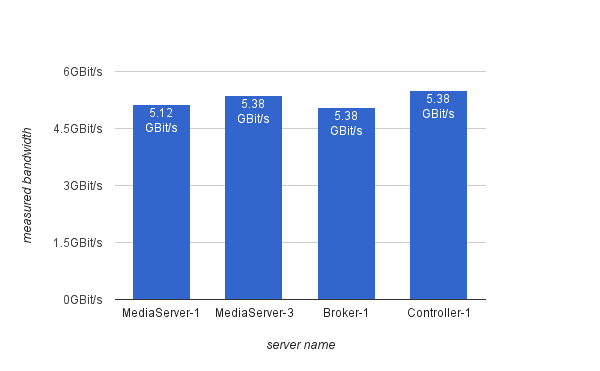
\includegraphics[width=0.5\textwidth]{images/evaluation/testbed_scenario2_bw}

\caption{Scenario 3: Bandwidth comparison}
\end{figure}

The first two bars show that the egress port on the Open vSwitch that the \textit{'MediaServer-3'} is connected to is limited to a combined bandwidth of 10 GBit/s. This is why the two connections share the available bandwidth and are nearly equal. It has to be remarked that the network performance is the average of a 10-second bandwidth test.

In the other QoS class the \textit{'MediaServer-2'} which is connecting to \textit{'Controller-1'} uses almost the full bandwidth of the available 1 GBit/s.

\textbf{UDP traffic}

The setup of iperf for generating the traffic is equal to Scenario 2.

\begin{table}[H]
\centering

\begin{tabularx}{\textwidth}{ |X|X|X|X|X| }
\hline Server name & Measured bandwidth & Ratio lost/total datagrams & Datagrams out of order & Jitter \\ 
\hline MediaServer-1 & 761 MBit/s & 5.9\% & 7 & 0.015 ms\\ 
\hline Controller-1 & 782 MBit/s & 3.5\% & 41 & 0.102 ms \\ 
\hline 
\end{tabularx}

\caption{Scenario 3: Network characteristics with generated UDP traffic}
\end{table}

The MediaServer-1 was connecting to the MediaServer-2 and the Controller-1 opened up a connection to Broker-1 in this case.

With having Quality of Service enabled with different rates, the difference in network statistics for UDP traffic is not very big. The only difference that is visible is that the Gold traffic of the MediaServer-1 is prioritized to the one of the Controller-1 which is part of the Wholesale QoS class.



\section{Conclusion}

The three test scenarios show an improvement of the network performance, which is given through placing the servers on a single host. Additionally with enabling Quality of Service, the network bandwidth for TCP traffic is shaped according to the requirements. It has been shown that the connection between Media Servers is prioritized to other service instance types. The Service-Level-Agreement of the Gold and Wholesale classes are fulfilled.